% Options for packages loaded elsewhere
\PassOptionsToPackage{unicode}{hyperref}
\PassOptionsToPackage{hyphens}{url}
%
\documentclass[
  12pt,
]{article}
\usepackage{amsmath,amssymb}
\usepackage{iftex}
\ifPDFTeX
  \usepackage[T1]{fontenc}
  \usepackage[utf8]{inputenc}
  \usepackage{textcomp} % provide euro and other symbols
\else % if luatex or xetex
  \usepackage{unicode-math} % this also loads fontspec
  \defaultfontfeatures{Scale=MatchLowercase}
  \defaultfontfeatures[\rmfamily]{Ligatures=TeX,Scale=1}
\fi
\usepackage{lmodern}
\ifPDFTeX\else
  % xetex/luatex font selection
    \setmainfont[]{TimesNewRoman}
\fi
% Use upquote if available, for straight quotes in verbatim environments
\IfFileExists{upquote.sty}{\usepackage{upquote}}{}
\IfFileExists{microtype.sty}{% use microtype if available
  \usepackage[]{microtype}
  \UseMicrotypeSet[protrusion]{basicmath} % disable protrusion for tt fonts
}{}
\makeatletter
\@ifundefined{KOMAClassName}{% if non-KOMA class
  \IfFileExists{parskip.sty}{%
    \usepackage{parskip}
  }{% else
    \setlength{\parindent}{0pt}
    \setlength{\parskip}{6pt plus 2pt minus 1pt}}
}{% if KOMA class
  \KOMAoptions{parskip=half}}
\makeatother
\usepackage{xcolor}
\usepackage[margin=1in]{geometry}
\usepackage{graphicx}
\makeatletter
\def\maxwidth{\ifdim\Gin@nat@width>\linewidth\linewidth\else\Gin@nat@width\fi}
\def\maxheight{\ifdim\Gin@nat@height>\textheight\textheight\else\Gin@nat@height\fi}
\makeatother
% Scale images if necessary, so that they will not overflow the page
% margins by default, and it is still possible to overwrite the defaults
% using explicit options in \includegraphics[width, height, ...]{}
\setkeys{Gin}{width=\maxwidth,height=\maxheight,keepaspectratio}
% Set default figure placement to htbp
\makeatletter
\def\fps@figure{htbp}
\makeatother
\setlength{\emergencystretch}{3em} % prevent overfull lines
\providecommand{\tightlist}{%
  \setlength{\itemsep}{0pt}\setlength{\parskip}{0pt}}
\setcounter{secnumdepth}{-\maxdimen} % remove section numbering
% definitions for citeproc citations
\NewDocumentCommand\citeproctext{}{}
\NewDocumentCommand\citeproc{mm}{%
  \begingroup\def\citeproctext{#2}\cite{#1}\endgroup}
\makeatletter
 % allow citations to break across lines
 \let\@cite@ofmt\@firstofone
 % avoid brackets around text for \cite:
 \def\@biblabel#1{}
 \def\@cite#1#2{{#1\if@tempswa , #2\fi}}
\makeatother
\newlength{\cslhangindent}
\setlength{\cslhangindent}{1.5em}
\newlength{\csllabelwidth}
\setlength{\csllabelwidth}{3em}
\newenvironment{CSLReferences}[2] % #1 hanging-indent, #2 entry-spacing
 {\begin{list}{}{%
  \setlength{\itemindent}{0pt}
  \setlength{\leftmargin}{0pt}
  \setlength{\parsep}{0pt}
  % turn on hanging indent if param 1 is 1
  \ifodd #1
   \setlength{\leftmargin}{\cslhangindent}
   \setlength{\itemindent}{-1\cslhangindent}
  \fi
  % set entry spacing
  \setlength{\itemsep}{#2\baselineskip}}}
 {\end{list}}
\usepackage{calc}
\newcommand{\CSLBlock}[1]{\hfill\break\parbox[t]{\linewidth}{\strut\ignorespaces#1\strut}}
\newcommand{\CSLLeftMargin}[1]{\parbox[t]{\csllabelwidth}{\strut#1\strut}}
\newcommand{\CSLRightInline}[1]{\parbox[t]{\linewidth - \csllabelwidth}{\strut#1\strut}}
\newcommand{\CSLIndent}[1]{\hspace{\cslhangindent}#1}
\ifLuaTeX
  \usepackage{selnolig}  % disable illegal ligatures
\fi
\usepackage{bookmark}
\IfFileExists{xurl.sty}{\usepackage{xurl}}{} % add URL line breaks if available
\urlstyle{same}
\hypersetup{
  pdftitle={Econometrics 343 - Empirical Analysis Project},
  hidelinks,
  pdfcreator={LaTeX via pandoc}}

\title{Econometrics 343 - Empirical Analysis Project}
\author{Luca Seazzu\\
\strut \\
Professor David Gebben}
\date{4/14/2023}

\begin{document}
\maketitle

\newcommand{\Prob}{\operatorname{Pr}}
\newcommand{\Binom}{\operatorname{Binom}}
\newcommand{\Unif}{\operatorname{Unif}}
\newcommand{\Triangle}{\operatorname{Triangle}}
\newcommand{\Norm}{\operatorname{Norm}}
\newcommand{\Beta}{\operatorname{Beta}}
\newcommand{\E}{\operatorname{E}}
\newcommand{\Var}{\operatorname{Var}}
\newcommand{\SD}{\operatorname{SD}}

\newpage

\subsection{Abstract:}\label{abstract}

~~In 2009, the Union of European Football Association (UEFA) determined
that more than half of 655 eligible European clubs incurred a net loss
over the previous year. While a small proportion were capable to sustain
heavy-losses year-to-year because of wealthy owners, it was determined
that at least 20\% of the clubs surveyed would be in financial peril
quickly while chasing success. Thus Financial Fair Play (FFP) was
created. The equation was that any money from the club's outgoing
transfers, employee benefits and wages, amortization of transfers,
finance costs, and dividends will be put again the club's income from
gate receipts, TV revenue, advertising, merchandising, disposal of
tangible fixed assets, finance, sales of players and prize money. All
money spent by the club on infrastructure, training facilities or youth
development will not be taken into account. Clubs are permitted to spend
up to five million euros more than they earn per three year assessment
period. However, big however, it can exceed that level to a limit if it
is covered by a direct contribution from the club's owner. (UEFA 2018)

~~Thus, this brings us to the question of what did FFP accomplish when
announced in 2009 and implemented in the 2013-2014 season? The economic
question is; did FFP implementation widen the gap between the wealthy
clubs and non-wealthy clubs based on their finishes in the standings
over the years? This is important because the goals of FFP were to make
it a more fair playing field, but to also ensure clubs don't bankrupt
themselves while chasing success. By showing 3 different linear
regression models that factor a club's income, position in the standings
from the prior year, their financial ranking according to Deloitte
Football Money League, and if the club is deemed one of the big six
clubs. The Deloitte Football Money League is ``an annual profile of the
highest revenue generating clubs in world football'' and they rank and
include analysis on the top 20-30 teams in the world. (Tim Bridge, Tom
Hammond, Alex Carr, Dhruv Garg, Alasdair Malcolm and Jenny Pang 2023)
The Premier League `Big 6' is an informal name for Arsenal, Chelsea,
Liverpool, Manchester City, Manchester United, and Tottenham Hotspur
because ``they are the most consistently successful teams in the
division\ldots{} {[}with{]} the biggest stadiums, broadest fan bases,
and the healthiest bank accounts.'' (Ryan Kelly 2021) These variables
should help correlate the effects of FFP on teams' success based on
their income, ranking, previous position, and the big 6.

\subsection{Model Fitting}\label{model-fitting}

~~Some data explanation. First, Income is measured in the millions of
euros. Rank is determined from 1 to 30 with 1 being the most income in
the world. Last\_Pos is determined by the team's position in the
standings at the end of the prior year, and Big6 is an indicator if the
club is one of Arsenal, Chelsea, Liverpool, Manchester City, Manchester
United, or Tottenham Hotspur. The year data is the year the season
ended, so 2009 means the 2008-2009 season and so on. Lastly, to clarify
the model, the lower the result, as long as greater than zero, the
better. The model is running a linear regression on Pos which is the
variable for the teams' standing in the current season, so they want to
be 1 which means they are on the top of the table/winning whereas 20
means they are at the bottom of the table/losing. The model is composed
of sums because the different variables are not interactive with each
other to justify any multiplication but it is rather a compilation of
the variables.

\subsubsection{Figure 1. 2001-2009 Linear Model
Summary}\label{figure-1.-2001-2009-linear-model-summary}

\begin{verbatim}
## MODEL INFO:
## Observations: 56 (16 missing obs. deleted)
## Dependent Variable: Pos
## Type: OLS linear regression 
## 
## MODEL FIT:
## F(4,51) = 17.530, p = 0.000
## R² = 0.579
## Adj. R² = 0.546 
## 
## Standard errors:OLS
## -------------------------------------------------------------
##                       Est.     2.5%    97.5%   t val.       p
## ----------------- -------- -------- -------- -------- -------
## (Intercept)          5.536   -0.361   11.433    1.885   0.065
## Income              -0.011   -0.032    0.011   -1.000   0.322
## Rank                 0.128   -0.099    0.355    1.134   0.262
## Last_Pos             0.316    0.045    0.587    2.344   0.023
## Big6                -1.922   -4.108    0.263   -1.766   0.083
## -------------------------------------------------------------
\end{verbatim}

\subsubsection{Figure 2. 2001-2009 Model Linear Regression
Post-Estimation
Plots}\label{figure-2.-2001-2009-model-linear-regression-post-estimation-plots}

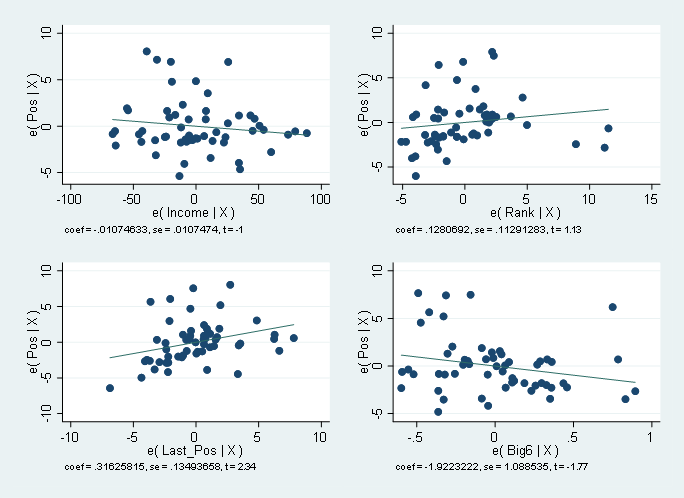
\includegraphics[width=450px]{2009}

\newpage

\subsubsection{Figure 3. 2010-2013 Linear Model
Summary}\label{figure-3.-2010-2013-linear-model-summary}

\begin{verbatim}
## MODEL INFO:
## Observations: 201 (33 missing obs. deleted)
## Dependent Variable: Pos
## Type: OLS linear regression 
## 
## MODEL FIT:
## F(4,196) = 70.072, p = 0.000
## R² = 0.588
## Adj. R² = 0.580 
## 
## Standard errors:OLS
## -------------------------------------------------------------
##                       Est.     2.5%    97.5%   t val.       p
## ----------------- -------- -------- -------- -------- -------
## (Intercept)          2.937    0.740    5.135    2.636   0.009
## Income               0.000   -0.003    0.004    0.097   0.923
## Rank                 0.207    0.113    0.300    4.359   0.000
## Last_Pos             0.291    0.159    0.424    4.323   0.000
## Big6                -1.790   -3.186   -0.395   -2.530   0.012
## -------------------------------------------------------------
\end{verbatim}

\subsubsection{Figure 4. 2010-2013 Model Linear Regression
Post-Estimation
Plots}\label{figure-4.-2010-2013-model-linear-regression-post-estimation-plots}

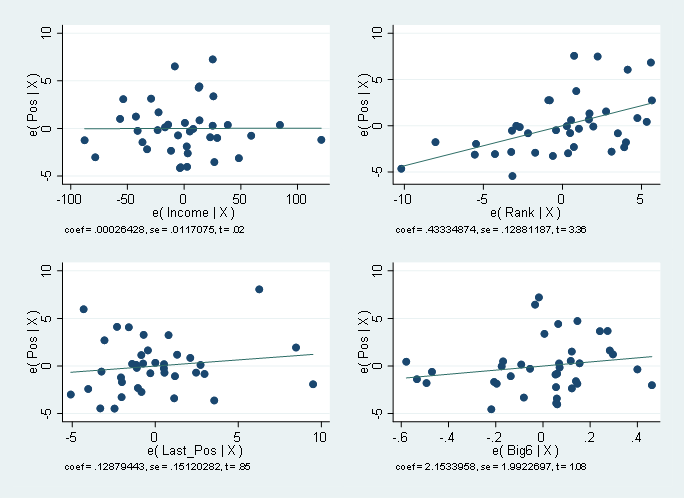
\includegraphics[width=450px]{2009.2013}

\newpage

\subsubsection{Figure 5. 2014-2022 Linear Model
Summary}\label{figure-5.-2014-2022-linear-model-summary}

\begin{verbatim}
## MODEL INFO:
## Observations: 107 (15 missing obs. deleted)
## Dependent Variable: Pos
## Type: OLS linear regression 
## 
## MODEL FIT:
## F(4,102) = 34.097, p = 0.000
## R² = 0.572
## Adj. R² = 0.555 
## 
## Standard errors:OLS
## -------------------------------------------------------------
##                       Est.     2.5%    97.5%   t val.       p
## ----------------- -------- -------- -------- -------- -------
## (Intercept)          6.739    1.482   11.996    2.543   0.013
## Income              -0.006   -0.015    0.003   -1.294   0.199
## Rank                 0.122   -0.042    0.286    1.472   0.144
## Last_Pos             0.230    0.029    0.431    2.266   0.026
## Big6                -1.457   -3.861    0.947   -1.202   0.232
## -------------------------------------------------------------
\end{verbatim}

\subsubsection{Figure 6. 2014-2022 Model Linear Regression
Post-Estimation
Plots}\label{figure-6.-2014-2022-model-linear-regression-post-estimation-plots}

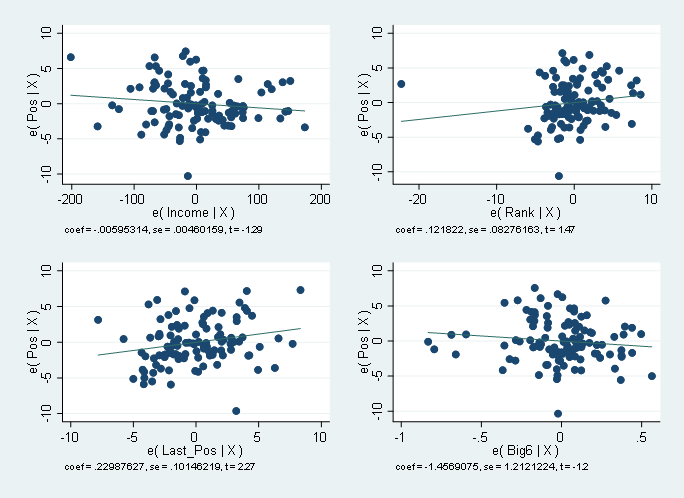
\includegraphics[width=450px]{2013}

\newpage

\subsection{Interpretation Of Models}\label{interpretation-of-models}

Figures 1 and 2 \textbar{} For the years 2001-2009 where FFP had not
been created or mentioned, the model produces an intercept of 5.543,
Income is -0.011, Rank is 0.128, Last\_Poss is 0.316, and Big6 is
-1.922. This means that Big6 is the highest indicator of a team having a
small position and therefore a better result. Income has a small
correlation towards a better position while also the higher Rank and
Last\_Poss are, the likelihood that Position will also be higher and
therefore bad.

Figures 3 and 4. \textbar{} For the years 2009-2013 where FFP had been
developed but not yet implemented, the model produces an intercept of
2.937, Income is 0, Rank is 0.207, Last\_Pos is 0.291, and Big6 is
-1.790. In comparison to 2001-2009, Income has slightly less effect than
before, the intercept is much different by almost 2.6 positional spots,
Rank has become about twice as important, the position from last season
remains about as important, and Big6 remains heavily important but not
quite as important as before.

Figures 5 and 6. \textbar{} For the years 2013 - 2022 where FFP has now
been fully implemented, the model produced an intercept of 6.739, wow!,
Income is -0.006, Rank is 0.122, Last\_Pos is 0.230, and Big6 is -1.457.
The intercept has increased a lot, even past the intercept for
2002-2009, Income is still around the same, Rank returned to its
influence from 2002-2009, Last\_Pos has decreased in influence again,
and Big6 has also decreased in influence again.

\subsection{F Test for
Heteroskedasticity}\label{f-test-for-heteroskedasticity}

\subsubsection{Figure 7. 2001-2009 Model
F-Test}\label{figure-7.-2001-2009-model-f-test}

\begin{verbatim}
## 
##  F Test for Heteroskedasticity
##  -----------------------------
##  Ho: Variance is homogenous
##  Ha: Variance is not homogenous
## 
##  Variables: fitted values of Pos 
## 
##        Test Summary         
##  ---------------------------
##  Num DF     =    1 
##  Den DF     =    54 
##  F          =    12.12082 
##  Prob > F   =    0.000995502
\end{verbatim}

\subsubsection{Figure 8. 2010-2013 Model
F-Test}\label{figure-8.-2010-2013-model-f-test}

\begin{verbatim}
## 
##  F Test for Heteroskedasticity
##  -----------------------------
##  Ho: Variance is homogenous
##  Ha: Variance is not homogenous
## 
##  Variables: fitted values of Pos 
## 
##         Test Summary         
##  ----------------------------
##  Num DF     =    1 
##  Den DF     =    199 
##  F          =    19.83003 
##  Prob > F   =    1.409637e-05
\end{verbatim}

\subsubsection{Figure 9. 2014-2022 Model
F-Test}\label{figure-9.-2014-2022-model-f-test}

\begin{verbatim}
## 
##  F Test for Heteroskedasticity
##  -----------------------------
##  Ho: Variance is homogenous
##  Ha: Variance is not homogenous
## 
##  Variables: fitted values of Pos 
## 
##       Test Summary        
##  -------------------------
##  Num DF     =    1 
##  Den DF     =    105 
##  F          =    5.779876 
##  Prob > F   =    0.0179626
\end{verbatim}

The F-Test for each model fails the assumption of heteroskedasticity
because the null hypothesis that the models are homogeneous must be
rejected at a p-value \textless{} 0.05.

\subsection{Ramsey RESET Test}\label{ramsey-reset-test}

\subsubsection{Figure 10. 2001-2009 Model Ramsey RESET
Test}\label{figure-10.-2001-2009-model-ramsey-reset-test}

\begin{verbatim}
## 
##  RESET test
## 
## data:  model09
## RESET = 2.4585, df1 = 4, df2 = 47, p-value = 0.05831
\end{verbatim}

\subsubsection{Figure 11. 2010-2013 Model Ramsey RESET
Test}\label{figure-11.-2010-2013-model-ramsey-reset-test}

\begin{verbatim}
## 
##  RESET test
## 
## data:  model09.13
## RESET = 0.4155, df1 = 4, df2 = 192, p-value = 0.7973
\end{verbatim}

\subsubsection{Figure 12. 2014-2022 Model Ramsey RESET
Test}\label{figure-12.-2014-2022-model-ramsey-reset-test}

\begin{verbatim}
## 
##  RESET test
## 
## data:  model13
## RESET = 1.2473, df1 = 4, df2 = 98, p-value = 0.2961
\end{verbatim}

Running the RESET Test on all three models shows p-values for the F-stat
at 5.8\%, 79.7\%, and 29.6\% which means we fail to rejest the Ramsey
RESET test null hypothesis. This indicates that the functional form is
correct and that the models do not suffer from omitted variables.

\newpage

\subsection{Implications}\label{implications}

~~The first point to mention is that each model failed the F Test for
Heteroskedasticity and thus these results are tainted slightly since
this means the population used in the regression contains unequal
variance and thus the analysis results may be invalid but not
necessarily. In hindsight, this may be due to the data being centered
around the Deloitte Football Money League and thus isn't taking into
account the teams that weren't among the richest in Europe for that
season. This would support the heteroskedasticity seen in the model and
would be something to do different if the models were recreated. If this
analyses were to be continued, the data should be redone and even more
interestingly expanded to contain the top 5 leagues of europe since most
of the 30 teams each year in the Deloitte Football Money League report
would be continued and see how they do comparitively. It would also be
interesting to add European tournament result of the clubs to see how
clubs do against each other rather than just their own league.

~~The results of the linear regressions models have some interesting
things to say about FFP. The first is that since FFP was announced and
then implemented, being one of the Big 6 has consistently decreased in
correlation to standing position and therefore maybe FFP is giving more
teams opportunity to finish above the Big 6 and thus more variability to
the league. Another interesting observation is the dip in the intercept
after FFP was announced but the massive spike back up after FFP was
implemented. This means that if all other values are 0, such as 0
income, no rank, no last position, and not part of the Big 6, teams
would on average be about 6.8 places behind other teams. This suggests
that the factors of more income, better rank and positioning, and being
part of the Big 6 has created more separation between the teams than
after FFP was announced but not yet implemented. This is interesting
because to hypothesize that when FFP was announced, it greatly effected
teams and made the playing field more even financially, as seen by the
model, but once it was implemented, it actually seemed to widen the gap
between the elite financially and those who aren't.

~~This economic question is important for the integrity of football
across the world because FFP should become more about giving teams equal
opportunity and chances rather than just the richest teams are always
the best. If it can be shown that richer teams on average have much more
success than their counterparts, something should be done about it for
the sake of the sport. It would also target one of the biggest problems
in football right now; inflated player transfer fees. Since FFP, player
transfer fees have skyrocketed because each team needs to balance their
financial books, but it has only snowballed out of control where even
somewhat normal players are being bought for 50-100 million euros a
piece. This is unhealthy for the sport and it has also become a place
where wealthy owners invest lots of money into wonder kids hoping to
sell them for profit in a few years. Overall this is unhealthy for the
sport and the longevity of true competition rather than wealthy
monopolies.

\newpage

\section*{References}\label{references}
\addcontentsline{toc}{section}{References}

\phantomsection\label{refs}
\begin{CSLReferences}{1}{0}
\bibitem[\citeproctext]{ref-Goal}
Ryan Kelly. 2021. \emph{Who Are the Premier League 'Big Six'? Top
English Clubs \& Nickname Explained}. Goal.
\url{https://www.goal.com/en-us/news/who-are-premier-league-big-six-top-english-clubs-nickname-explained/130iokmi8t8dt1k3kudou73s1k}.

\bibitem[\citeproctext]{ref-Deloitte}
Tim Bridge, Tom Hammond, Alex Carr, Dhruv Garg, Alasdair Malcolm and
Jenny Pang. 2023. \emph{Deloitte Football Money League}. Deloitte,
Deloitte Sports Business Group.
\url{https://www2.deloitte.com/uk/en/pages/sports-business-group/articles/deloitte-football-money-league.html}.

\bibitem[\citeproctext]{ref-UEFA}
UEFA. 2018. \emph{UEFA Club Licensing and Financial Fair Play
Regulations}. UEFA.
\url{https://documents.uefa.com/v/u/MFxeqLNKelkYyh5JSafuhg}.

\end{CSLReferences}

\end{document}
